\chapter{Arktitektur}
Dette kapitel viser arkitekturen for Rambøll Tilsyn. \\ \\ \label{sec:Arkitektur}
På figur \ref{fig:OversigtSystembeskrivelse} ses oversigten over systemet og hvordan de forskellige elementer forbinder hinanden i systemet.
\begin{figure}[H] % (alternativt [H])
	\centering
	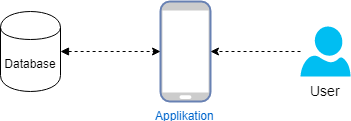
\includegraphics[height=3cm, width=8cm]{../ArkitekturDesign/OverordnetArkitektur//Oversigtoversystem}
	\caption{Oversigt over systemet.}
	\label{fig:OversigtSystembeskrivelse}
\end{figure}
Det ses på figur \ref{fig:OversigtSystembeskrivelse}, at brugeren benytter applikationen. Applikationen kommunikere så via internettet til databasen. \\
Yderligere beskrivelse af systemet kan findes i afsnit \ref{Krav-sec:Systembeskrivelse} Systembeskrivelse i kravspecifikationen som er vedlagt i bilag.

\clearpage

\section{Domænemodel}
En domænemodel giver et overblik over, hvordan systemmet skal bygges op. Domænemodellen viser forbindelserne mellem forskellige elementer i systemmet, og hvordan de interagerer med hinanden. Dette gør det lettere at gå fra domænen til implementation.
I dette projekt er der udarbejdet én domænemodel som ses på figur \ref{fig:Domain}.

\begin{figure}[H] % (alternativt [H])
	\centering
	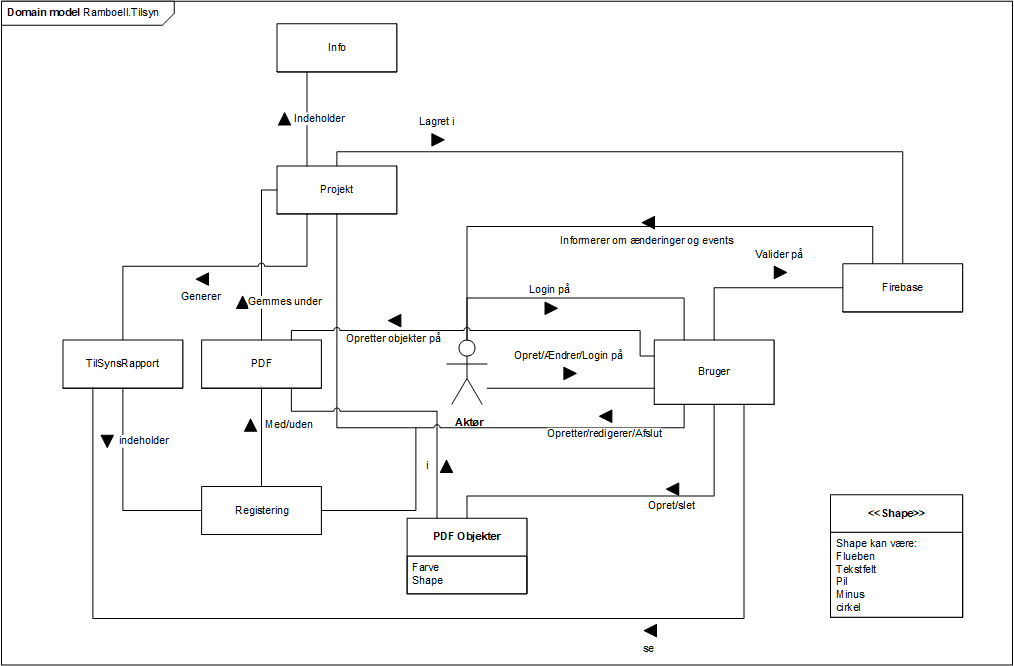
\includegraphics[height=13cm, width=17cm]{../ArkitekturDesign/OverordnetArkitektur/Domainmodel}
	\caption{Domænemodel for Rambøll Tilsyn.}
	\label{fig:Domain}
\end{figure}
Brugeren logger ind på applikationen. Her kan bruger så oprette et projekt, som vil indeholde en registrering. I denne registrering kan bruger tilknytte en PDF tegning. På PDF tegningen kan brugeren oprette forskellige objekter, eller fjerne forkerte objekter. \\
Når bruger er færdig med en registrering, vil objekter, PDF tegning mv. blive gemt i Firebase databasen.

\clearpage